\begin{answer}
	\begin{figure}[H]
		\centering
		\begin{subfigure}[H]{0.45\linewidth}
			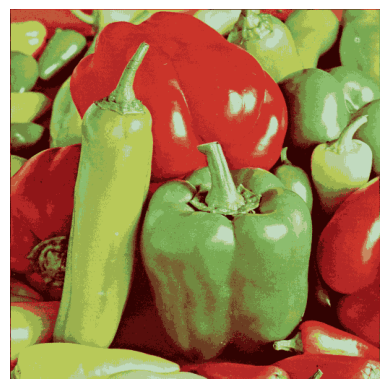
\includegraphics[width=\linewidth]{updated_large.png}
			\caption{The compressed image.}
		\end{subfigure}
		\begin{subfigure}[H]{0.45\linewidth}
			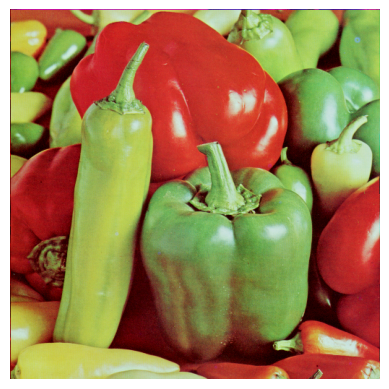
\includegraphics[width=\linewidth]{orig_large}
			\caption{The original image.}
		\end{subfigure}
		\caption{K-means for image compression.}
	\end{figure}
\end{answer}
